\documentclass{beamer}

\usepackage[english]{babel}
\usepackage[utf8x]{inputenc}
\usepackage[inline]{asymptote}
\usepackage{slide_helper}
\usepackage{tikz}
\usepackage{circuitikz}
\usetikzlibrary{calc,patterns,decorations.pathmorphing,decorations.markings}

%\hideasymptote% uncomment to not compile asymptote graphs

\title[MATH 2250 - Section 4.1]{The Harmonic Oscillator}

\begin{document}

\begin{frame}
  \titlepage
\end{frame}

\begin{frame}
\begin{block}{Newton's Dot Notation}
Scientists and Engineers who work with many variables where the independent variables is always $t$ commonly use dot notation:
\begin{equation*}
\ndot{x}{1}=\dfrac{dx}{dt}
\quad\text{and}\quad
\ndot{x}{2}=\dfrac{dx^2}{d^2t}
\quad\text{and}\quad
\ndot{x}{3}=\dfrac{dx^3}{d^3t}
\quad\text{and}\quad
\ndot{x}{4}=\dfrac{dx^4}{d^4t}
\end{equation*}
\end{block}\pause

\begin{definition}
A very important DE is the second-order homogeneous equation
\begin{equation*}
m\ndot{x}{2}+b\ndot{x}{1}+kx=0
\end{equation*}
where $m>0$, $b$, and $k$ are constants.

This models a class of phenomena called \textbf{damped harmonic oscillation}.  
\end{definition}
\end{frame}

\begin{frame}
\begin{block}{The Mass-Spring System}
\begin{columns}
\begin{column}{0.4\textwidth}
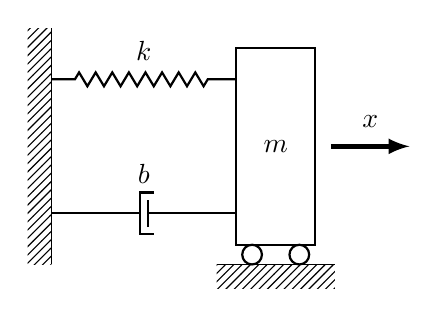
\begin{tikzpicture}[every node/.style={draw,outer sep=0pt,thick}]
\tikzstyle{spring}=[thick,decorate,decoration={zigzag,pre length=0.3cm,post length=0.3cm,segment length=6}]
\tikzstyle{damper}=[thick,decoration={markings,  
  mark connection node=dmp,
  mark=at position 0.5 with 
  {
    \node (dmp) [thick,inner sep=0pt,transform shape,rotate=-90,minimum width=15pt,minimum height=3pt,draw=none] {};
    \draw [thick] ($(dmp.north east)+(2pt,0)$) -- (dmp.south east) -- (dmp.south west) -- ($(dmp.north west)+(2pt,0)$);
    \draw [thick] ($(dmp.north)+(0,-5pt)$) -- ($(dmp.north)+(0,5pt)$);
  }
}, decorate]
\tikzstyle{ground}=[fill,pattern=north east lines,draw=none,minimum width=0.75cm,minimum height=0.3cm]

\node (M) [minimum width=1cm, minimum height=2.5cm] {$m$};

\node (ground) [ground,anchor=north,yshift=-0.25cm,minimum width=1.5cm] at (M.south) {};
\draw (ground.north east) -- (ground.north west);
\draw [thick] (M.south west) ++ (0.2cm,-0.125cm) circle (0.125cm)  (M.south east) ++ (-0.2cm,-0.125cm) circle (0.125cm);

\node (wall) [ground, rotate=-90, minimum width=3cm,yshift=-3cm] {};
\draw (wall.north east) -- (wall.north west);

\draw [spring] (wall.170) -- ($(M.north west)!(wall.170)!(M.south west)$) node [draw=none, midway, label=above:{$k$}] {};
\draw [damper] (wall.10) -- ($(M.north west)!(wall.10)!(M.south west)$) node [draw=none, midway, label={[label distance=.15cm]90:$b$}] {};

\draw [-latex,ultra thick] (M.east) ++ (0.2cm,0) -- +(1cm,0) node [draw=none, midway, label=above:{$x$}] {};
\end{tikzpicture}
\end{column}
\begin{column}{0.55\textwidth}
We will model the Mass-Spring system using Newton's Second Law of Motion, $F=m\ndot{x}{2}$, where $F$ is the sum of the following forces:
\onslide<+->
\begin{itemize}[<+- | alert@+>]
\item The restoring force of the spring. \\ $F_{\text{restoring}}=-kz$ where $k>0$
\item The damping force. \\ $F_{\text{damping}}=-bx$ where $b\geq0$
\item Any external \quotetext{driving} forces. $F_{\text{external}}=f(t)$ where $f(t)$ is the sum of all external forces.
\end{itemize}
\end{column}
\end{columns}
\onslide<+->
\vspace{4mm}
Summing these forces gives:
\begin{tabular}{rlll}
mass $\times$ acceleration &= $F_{\text{restoring}}$ &+ $F_{\text{damping}}$ &+ $F_{\text{external}}$\\
$m\ndot{x}{2}$ &= $-kx$ &- $b\ndot{x}{1}$ &+ $f(t)$
\end{tabular}
\end{block}
\end{frame}

\begin{frame}
\begin{block}{Simple Harmonic Oscillator}
The simple harmonic oscillator equation is
\begin{equation*}
m\ndot{x}{2} +b\ndot{x}{1}+kx=f(t)
\end{equation*}
with constant coefficients $m>0$, $k>0$, and $b\geq 0$.

\onslide<+->
\begin{itemize}[<+- | alert@+>]
\item When $b=0$, the motion is called \textbf{undamped}; otherwise it is \textbf{damped}.
\item If $f(t)=0$ for all $t$, then the equation is homogeneous:
\begin{equation*}
m\ndot{x}{2} +b\ndot{x}{1}+kx=0
\end{equation*}
and the motion is called \textbf{unforced}, \textbf{undriven}, or \textbf{free}; otherwise it is called \textbf{forced} or \textbf{driven}. 
\end{itemize}
\end{block}
\end{frame}

\begin{frame}
\begin{example}
\begin{overprint}
\onslide<1-3>
Let us consider a mass of 1~kg resting on a table that is attached to the wall by a spring.
\visible<2->{

\vspace{2mm}
We discover that it takes a force of 1 newton to push the mass 0.25 meters from it's resting position.
\begin{equation*}
k=\dfrac{1~\text{newton}}{0.25~\text{meter}}=4~\dfrac{\text{newton}}{\text{meter}}
\end{equation*}}
\visible<3->{We also measure the damping force of the object sliding on the table to be 0.5 newtons when the velocity is 0.25 meters per second.
\begin{equation*}
b=\dfrac{0.5~\text{newton}}{0.25~\dfrac{\text{meter}}{second}}=2~\dfrac{\text{newton second}}{\text{meter}}
\end{equation*}}
\onslide<4->
The object is pulled to the right until the spring is stretched 0.5 meters and then released. (The motion is unforced.)
\visible<5->{%

\vspace{2mm}
So, the initial conditions are
\begin{equation*}
x(0)=0.5~\text{meters}
\quad\text{and}\quad
\ndot{x}{1}(0)=0~\dfrac{\text{meter}}{\text{second}}
\end{equation*}}
\visible<6->{We can now formulate the IVP that describes this system
\begin{center}
\begin{tabular}{rlllll}
$m\ndot{x}{2}$&$+b\ndot{x}{1}$&$+kx$&$=f(t)$&&\\
\visible<7->{$\ndot{x}{2}$&$+2\ndot{x}{1}$&$+4x$&$=0$&$x(0)=0.5$,& $\ndot{x}{1} (0)=0$}
\end{tabular}
\end{center}}
\visible<8->{Notice that a second-order DE requires \textbf{two} initial conditions.}
\end{overprint}
\end{example}
\end{frame}

\begin{frame}
\begin{block}{Systems of Units}
There are three systems of units you are likely to encounter:
\onslide<+->
\begin{itemize}[<+- | alert@+>]
\item \textbf{International System of Units (SI)}.
\item \textbf{Centimetre-Gram-Second system of units}, a precursor to SI\@.
\item \textbf{United States customary units}, the variant of Imperial Units that the United States uses.
\end{itemize}
\end{block}
\onslide<+->
\begin{block}{Units of measure}
\begin{tabular}{llll}
\textbf{Quantity} & \textbf{SI} & \textbf{CGS} & \textbf{US Customary} \\
\hline
Force & newton (N) & dyne & pound (lb) \\
\onslide<+->
Mass & kilogram (kg) & gram (gm) & slug (lb sec\textasciicircum2/ft) \\
\onslide<+->
Length & meter (m) & centimeter (cm) & foot (ft) \\
\onslide<+->
Energy & joule & erg & foot-pound (ft-lb) \\
\onslide<+->
Gravity (Earth) & 9.8 $\dfrac{\text{m}}{{\text{s}}^2}$ & 980.665 $\dfrac{\text{cm}}{{\text{s}}^2}$ & 32 $\dfrac{\text{ft}}{{\text{s}}^2}$
\end{tabular}
\end{block}
\end{frame}

\begin{frame}
\begin{example}
We can guess a solution to
\begin{equation*}
m\ndot{x}{2}+kx=0
\end{equation*}\pause
We know that ${\left(\sin[t]\right)}^{\prime\prime}=-\sin[t]$ and ${\left(\cos[t]\right)}^{\prime\prime}=-\cos[t]$. So, a solution to the DE is probably going to contain sines and cosines.\pause

\vspace{2mm}
Comparing
\begin{equation*}
{\left(\sin[\omega_0 t]\right)}^{\prime\prime}=-\omega_0^2\sin[\omega_0 t]
\quad\text{and}\quad
\ndot{x}{2}=-\dfrac{k}{m}x
\end{equation*}
we see that if $\omega_0=\sqrt{\dfrac{k}{m}}$, then $x(t)=\sin[\omega_0 t]$ is a solution.
\end{example}\pause
\begin{block}{Note}
Another solutions is $x(t)=\cos[\omega_0 t]$.
\end{block}
\end{frame}

\begin{frame}
\begin{block}{Solution of the Undamped Unforced Oscillator}
For the undamped unforced oscillator
\begin{equation*}
m\ndot{x}{2}+kx=0
\end{equation*}
we know two solutions:
\begin{equation*}
x(t)=\cos[\omega_0 t]
\quad\text{and}\quad
x(t)=\sin[\omega_0 t]
\quad\text{where}\quad
\omega_0=\sqrt{\dfrac{k}{m}}
\end{equation*}\pause
The Superposition Principle tells us that any linear combination of these two solutions is itself a solution. Thus, for $c_1,c_2\in\R$, the family of solutions is
\begin{equation*}
x(t)=c_1\cos[\omega_0 t]+c_2\sin[\omega_0 t]
\end{equation*}
\end{block}\pause
\begin{block}{Note}
We will see next section that these cover all solutions.
\end{block}
\end{frame}

\begin{frame}
\onslide<+->
\begin{block}{Alternate Form of the Undamped Unforced Oscillator Solution}
Solutions to the undamped unforced oscillator may also be expressed as
\begin{equation*}
x(t)=A\cos[\omega_0 t-\delta]
\end{equation*}

\vspace{-0.5cm}
\begin{dynitemize}[<+- | alert@+>]
\item $A$ is the \textbf{amplitude}.
\item $\delta$ is the \textbf{phase angle}, measured in radians.
\item The motion has \textbf{circular frequency} $\omega_o=\sqrt{\dfrac{k}{m}}$, measured in $\dfrac{\text{radians}}{\text{second}}$.
\item The \textbf{natural frequency} is $f_0=\dfrac{\omega_0}{2\pi}$.
\item The \textbf{period} is $\dfrac{1}{f_0}=\dfrac{2\pi}{\omega_0}=2\pi\sqrt{\dfrac{m}{k}}$, measured in seconds.
\item This is a horizontal translation of $A\cos[\omega_o t]$ with \textbf{phase shift} $\dfrac{\delta}{\omega_0}$.
\end{dynitemize}
\end{block}
\end{frame}

\begin{frame}
\begin{block}{Converting Between the Two Forms}
The translation is given by
\begin{equation*}
A=\sqrt{c_1^2+c_2^2},\qquad\tan[\delta]=\dfrac{c_2}{c_1}
\end{equation*}
and
\begin{equation*}
c_1=A\cos[\delta],\qquad c_2=A\sin[\delta]
\end{equation*}
\end{block}
\end{frame}

\begin{frame}
\begin{example}
Let us solve the following second-order IVP\@.
\begin{equation*}
\ndot{x}{2}+x=0,\quad
x(0)=0,\quad
\ndot{x}{1}(0)=1
\end{equation*}\pause
So, $m=1$, $k=1$, and $\omega_0=\sqrt{\dfrac{1}{1}}=1$.\pause

\vspace{2mm}
The general solution is
\begin{equation*}
x(t)=c_1\cos[t]+c_2\sin[t]
\end{equation*}\pause
Differentiating gives
\begin{equation*}
\ndot{x}{1}=-c_1\sin[t]+c_2\cos[t]
\end{equation*}\pause
Substituting $t=0$, $x(0)=0$, and $\ndot{x}{1}(0)=1$ into this system gives the solution $c_1=0$ and $c_2=1$.
\end{example}
\end{frame}

\begin{frame}[fragile]
\begin{example}
Let us look at some plots concerning $\ndot{x}{2}+0.25x=0$:

\begin{center}
\begin{columns}
\begin{column}{.5\textwidth}
\centering
\begin{asy}
import graph;
import fontsize;
defaultpen(fontsize(9pt));
size(170);
real min_x=-pi/2, max_x=7pi;
real min_y=-5, max_y=5;

for (real c=0.75; c <= 2.0; c+=0.25)
{
	real omega=0.5;
	real delta=pi/2;
	real A=c/(omega*sin(delta));
	real f(real x) {return A*cos(omega*x-delta);}
	draw(graph(f,min_x, max_x),blue+0.5bp);
}

xaxis("$t$",YEquals(0),min_x,max_x,NoTicks());
yaxis("$x$",XEquals(0),min_y,max_y,NoTicks());
\end{asy}
\end{column}
\begin{column}{.5\textwidth}
\centering
\begin{asy}
import graph;
import fontsize;
defaultpen(fontsize(9pt));
size(170);
real min_x=-pi/2, max_x=7pi;
real min_y=-5, max_y=5;

for (real c=0.75; c <= 2.0; c+=0.25)
{
	real omega=0.5;
	real delta=pi/2;
	real A=c/(omega *sin(delta));
	real f(real x) {return -1*omega*A*sin(omega*x-delta);}
	draw(graph(f,min_x, max_x),blue+0.5bp);
}

xaxis("$t$",YEquals(0),min_x,max_x,NoTicks());
yaxis("$\dot{x}$",XEquals(0),min_y,max_y,NoTicks());
\end{asy}
\end{column}
\end{columns}
\begin{asy}
import graph;
import slopefield;
import fontsize;
defaultpen(fontsize(9pt));
size(145);
real min_x=-6, max_x=6;
real min_y=-6, max_y=6;
pair a=(min_x,min_y);
pair b=(max_x,max_y);

real length(real x, real y) {return (x == 0) && (y == 0) ? 0.0001 : sqrt(x*x+y*y);}
path vector(pair z) {return (0,0)--1/(2*length(z.y,-0.25*z.x))*(z.y,-0.25*z.x);}

add(vectorfield(vector,a,b,arrow=EndArrow(SimpleHead)));

real f(real dx, real ddx) {return -0.25*ddx;}

for(real gx=min_x+1; gx<=max_x-1; ++gx)
	draw((gx,min_y)--(gx,max_y),dotted+darkgray);
    
for(real gy=min_y+1; gy<=max_y-1; ++gy)
	draw((min_x,gy)--(max_x,gy),dotted+darkgray); 

xaxis("$x$",YEquals(min_y),min_x,max_x,NoTicks());
xaxis(YEquals(max_y),min_x,max_x);
yaxis("$\dot{x}$",XEquals(min_x),min_y,max_y,NoTicks());
yaxis(XEquals(max_x),min_y,max_y);
\end{asy}
\end{center}
\end{example}
\end{frame}

\begin{frame}
\begin{block}{Phase Portraits}
For any autonomous second-order differential equation
\begin{equation*}
\ndot{x}{2}=F\left(x,\ndot{x}{1}\right)
\end{equation*}
the \textbf{phase plane} is the two-dimensional graph with $x$ and $\ndot{x}{1}$ axes.\pause

\vspace{2mm}
The phase plane has a \textbf{vector field} specified by the DE, which at any point in the phase plane gives a direction vector with
\begin{center}
\begin{tabular}{rl}
horizontal component & $dx/dt=\ndot{x}{1}$ \\
\vspace{2mm}
vertical component & $d\ndot{x}{1}/dt=\ndot{x}{2}$
\end{tabular}
\end{center}\pause
\vspace{-2mm}
A \textbf{trajectory} is a path formed parametrically by the DE solutions $x(t)$ and $\ndot{x}{1}(t)$ as they follow the vector field. A graph showing phase plane trajectories is called a \textbf{phase portrait}.
\end{block}\pause
\begin{block}{Note}
Phase portraits can be graphed \emph{without} solving the DE\@.
\end{block}
\end{frame}

\begin{frame}
\begin{definition}
The second-order differential equation
\begin{equation*}
m\ndot{x}{2}+b\ndot{x}{1}+kx=f(t)
\end{equation*}
is equivalent to the system of first-order equations:
\begin{center}
\begin{tabular}{rl}
$\ndot{x}{1}$ &$= y$ \\
$\ndot{y}{1}$ &$= \ndot{x}{2} = \dfrac{f(t)}{m}-\dfrac{k}{m}x-\dfrac{b}{m}y$
\end{tabular}
\end{center}
\end{definition}\pause

\begin{example}
To draw the vector field for $\ndot{x}{2}+0.25x=0$ we can build the system:\pause
\begin{center}
\begin{tabular}{rl}
$\ndot{x}{1}$ &$= y$ \\
$\ndot{y}{1}$ &$= 0.25x$
\end{tabular}
\end{center}\pause
\vspace{-2mm}
Then, pplane may be used to plot the phase portrait.
\end{example}
\end{frame}

\begin{frame}
\begin{block}{Electrical Circuits}
\usepercentframe{0.7}{%
\begin{columns}
\begin{column}{0.25\textwidth}
\begin{circuitikz} \draw
(0,4) to[esource, l=$V(t)$, i=$I(t)$] (0,0)
      to[C, l=$C$] (2,0) 
      to[R, l_=$R$] (2,4)
      to[L, l=$L$] (0,4)
;
\end{circuitikz}
\end{column}
\begin{column}{0.55\textwidth}
\only<1-2>{

The current $I$ in a wire, measured in \emph{amperes}, is the flow of charge $Q$. That is, the current is the rate of change of the charge
\begin{equation*}
I(t)=\ndot{Q}{1}(t)
\end{equation*}
\visible<2->{

\vspace{-4mm}
\textbf{Kirchoff's Voltage Law} tell us that the input voltage $V(t)$ is the sum of voltage drops around the circuit. In our circuit, we have three such voltage drops.}}
\only<3>{

\textbf{Drop across a Resistor:} By \textbf{Ohm's Law}, the voltage drop across a resistor is proportional to the current passing through it.
\begin{equation*}
V_R(t)=R\cdot I(t)
\end{equation*}
Where $R$ is the \textbf{resistance} of the resistor and is measured in \emph{ohms}.}
\only<4>{

\textbf{Drop across an Inductor:} By \text{Faraday's Law}, the voltage drop across an inductor is proportional to the time rate of change of the current passing through it.
\begin{equation*}
V_L(t)=L\cdot\ndot{I}{1}(t)
\end{equation*}
where $L$ is the \textbf{inductance} and is measured in \emph{henries}.}
\only<5>{

\textbf{Drop across a Capacitor:} The voltage drop across a capacitor is proportional to the charge $Q(t)$ on the capacitor.
\begin{equation*}
V_C(t)=\dfrac{1}{C}Q(t)=\dfrac{1}{C}\int I(t)dt
\end{equation*}
where $C$ is the \textbf{capacitance} of the capacitor and is measured in \emph{farads}.}
\only<6>{

Thus, the voltage drop across the circuit is
\begin{equation*}
V(t)=R\cdot I+L\cdot\ndot{I}{1}+\dfrac{1}{C}\int I(t)dt
\end{equation*}
This is called an \textbf{integro-differential equation} because it contains both a derivative and an integral.}
\end{column}
\end{columns}}
\end{block}
\end{frame}

\begin{frame}
\begin{block}{}
Using the fact that $I(t)=\ndot{Q}{1}(t)$ we can build the following equations.
\end{block}\pause
\begin{block}{Series Circuit Equation (Charge)}
\begin{equation*}
\vspace{-1mm}
L\ndot{Q}{2}+R\ndot{Q}{1}+\dfrac{1}{C}Q=V(t)
\end{equation*}
If there is no voltage source ($V(t)=0$), then
\vspace{-2mm}
\begin{equation*}
L\ndot{Q}{2}+R\ndot{Q}{1}+\dfrac{1}{C}Q=0
\end{equation*}
\end{block}\pause
\begin{block}{Series Circuit Equation (Current)}
\begin{equation*}
L\ndot{I}{2}+R\ndot{I}{1}+\dfrac{1}{C}I=\ndot{V}{1}(t)
\end{equation*}
\vspace{-1mm}
If there is no voltage source ($V(t)=0$), then
\vspace{-2mm}
\begin{equation*}
L\ndot{I}{2}+R\ndot{I}{1}+\dfrac{1}{C}I=0
\end{equation*}
\end{block}
\end{frame}

\begin{frame}
\begin{example}
\begin{columns}
\begin{column}{0.25\textwidth}
\begin{circuitikz} \draw
(0,4) to[esource, l=$V(t)$, i=$I(t)$] (0,0)
      to[C, l=$C$] (2,0) 
      to           (2,4)
      to[L, l=$L$] (0,4)
;
\end{circuitikz}
\end{column}
\begin{column}{0.55\textwidth}
Consider a circuit composed of a capacitor and inductor hooked up in series. Suppose that at $t=0$ a charge $Q_0$ is put on the capacitor.\pause

\vspace{2mm}
The IVP is
\begin{equation*}
L\ndot{Q}{2}+\dfrac{1}{C}=0,\quad Q(0)=Q_0,\quad \ndot{Q}{1}(0)=0
\end{equation*}\pause
Thus, the solution is 
\begin{equation*}
Q(t)=c_1\cos[\omega_0 t]+c_2\sin[\omega_0 t]
\end{equation*}
where
\begin{equation*}
\omega_0=\sqrt{\dfrac{1}{LC}}
\end{equation*}
\end{column}
\end{columns}
\end{example}
\end{frame}
\end{document}

